\chapter{Design}

In this chapter, we properly introduce Psnodig and relevant design decisions behind the tool. We also describe the design behind the Gourmet programming language, as well the desicions behind the writers we landed on.

\section{Proposed Solution}

To solve the problem we are dealing with, we introduce Psnodig. We believe that Psnodig offers something unique in the context of this problem. Psnodig is a transpiler, first and foremost intended to convert executable programs to equivalent presentation-only programs. \\

The software discussed in Section 3.3 all do a very good job in their own right. The effort invested by developers, researchers and others involved is clearly reflected in both functionality and performance in each application. \\

However, the results they generate are sealed, and we have no choice but to accept whatever we receive. We believe there is more value in a tool that also lets us modify the final result, in case the translation from source code to PDF is ultimately too lossy. \\

Additionally, we also believe these writers actually lie in the same sphere. Thus, it would make sense to gather and apply them in the same tool, rather than having to switch between different ones. Lastly, we see value in users adding their own parsers and code generators, to further increase the tool's usefulness. \\

As the programs discussed in Section 3.3 primarily specialise in code generation, the DSLs are not actually executable. We believe that this is something that could be of tremendous use, and have therefore incorporated an interpreter that works on the internal representation of Psnodig. To the best of our knowledge, a tool which combines these exact devices does not currently exist.

\section{Psnodig}

Psnodig is a collection of data types in Haskell, describing a computer program. As such, it does not provide a lot of functionality on its own. It is first when we add parsers and writers that it shows its usefulness. \\

Since we are free to add parsers and writers at will, only our imagination (and programming abilities) can limit what we use it to convert. However, it is first and foremost intended as a tool for converting executable source programs to a presentation-only target programs. \\

Psnodig's transpilation flow is as follows: source programs are parsed to an internal, intermediate representation. Later, this representation is used to convert the original program further to a new target program. This means that a source program written in different languages can produce the same target program, given that their ASTs are identical. \\

Psnodig also comes with an interpreter, which works on the internal representation. This means that we can add parsers and run the code, without also having to write an interpreter or compiler. \\

All of this leads to a feeling of predictability: We write our source code in an available language. Then we use the interpreter to test it, until we are satisfied with the results. Now we are able to transpile it to TBP and IBP through the command line, rather than having to reconstruct it all manually. \\

Currently, Psnodig offers multiple command line arguments. If we at some point wish to add more, we can add them to the project's \texttt{Main.hs} file. The available command line arguments are the following: \\

\texttt{stack run program}, which parses a program and runs it through the interpreter. If our program contains any reachable print-statements, their arguments will be printed back to the command line. \\

\texttt{stack run ast program}, which prints the program's AST to the terminal, given that the program is syntactically correct. This can be a nice way to debug programs, and get a better understanding of how our parsers actually parse our programs. \\

\texttt{stack run tbp program}, which parses the program and produces a LaTeX file containing the program's TBP version. We can also add a flag \texttt{pdf} after \texttt{tbp} to get a PDF of the compiled LaTeX file. \\

\texttt{stack run ibp program}, which parses the program and produces a LaTeX file containing the program's IBP version. We can also add a flag \texttt{pdf} after \texttt{ibp} to get a PDF of the compiled LaTeX file. \\

\texttt{stack run gourmet program}, which parses a Gourmet program to an intermediate representation, before writing it back to the original Gourmet code. It is mainly intended for purposes of testing Psnodig's consistency.

\subsection{Syntax}

To present Psnodig's grammar, we have decided to go with EBNF, as shown in \Cref{Psnodig's EBNF.}. EBNF, short for Extended Backus-Naur form, is a simple, precise and sufficiently powerful notation to formally describe the syntax of a programming language~\cite{feynman2016ebnf}. We could have opted for the original BNF notation, but EBNF allows us to present it more suffinctly. \\

\Cref{Meta symbols used to describe Psnodig's grammar.} shows the meta symbols we use to help describe the grammar. Arrows indicate the application of a rule. Curly brackets indicate repetition of 0 or more times (much like the reflexive arrow in \Cref{An example finite state automata.}). Square brackets indicate binary presentness. Vertical bars indicate disjunction, like we saw in Section 2.2.1. \\

\begin{lstlisting}[caption={Meta symbols used to describe Psnodig's grammar.}, captionpos=b, label={Meta symbols used to describe Psnodig's grammar.}]
-> { } [ ] |
\end{lstlisting}

Non-terminals are written in upper case. There are also five terminals written in upper case, that do not have production rules. \texttt{NAME}, which works as a placeholder for an identifier, e.g. the name of a function. \texttt{INTEGER}, which is any $n \in \mathbb{N}$. \texttt{DECIMAL}, which is any $q \in \mathbb{Q}$. \texttt{BOOLEAN}, which is a $b \in \{\top, \bot \}$. Lastly, \texttt{NIL} is meant to indicate the absence of a value. \\

\forsup{Bør jeg forklare dette mer? F.eks. dette med terminals og non-terminals osv, production rules etc.}

\begin{lstlisting}[caption={Psnodig's grammar in EBNF notation.}, captionpos=b, label={Psnodig's EBNF.}]
PROGRAM            -> [ PROGRAMDESCRIPTION ] { STRUCTDECL }
                      { FUNCTIONDECL } [ FUNCTIONCALL ]

PROGRAMDESCRIPTION -> NAME NAME

STRUCTDECL         -> NAME { ARGUMENT }

STRUCT             -> NAME { EXPRESSION }

STRUCTFIELD        -> EXPRESSION EXPRESSION

FUNCTIONDECL       -> NAME { ARGUMENT } { Statement }

ARGUMENT           -> ARGUMENT NAME NAME

STATEMENT          -> ASSIGNMENT | LOOP | IF | FOREACH | FOR
                      | FUNCTIONCALL | RETURN | HASHSTMT
                      | ANNOTATIONSTMT | Break | Continue

ASSIGNMENT         -> ASSIGNMENTTARGET ASSIGNMENTVALUE

LOOP               -> EXPRESSION { STATEMENT }

IF                 -> EXPRESSION { STATEMENT } [ ELSE ]

FOREACH            -> NAME EXPRESSION { STATEMENT }

FOR                -> NAME EXPRESSION EXPRESSION { STATEMENT }

FUNCTIONCALL       -> NAME [EXPRESSION]

RETURN             -> EXPRESSION

HASHSTMT           -> STATEMENT

ANNOTATIONSTMT     -> NAME { STATEMENT }

ASSIGNMENTTARGET   -> NAME | LISTINDEX | STRUTFIELD

ASSIGNMENTVALUE    -> EXPRESSION | STRUCT

ELSE               -> IF | { STATEMENT }

EXPRESSION         -> VALUE | NAME
                      | OPERATOR EXPRESSION EXPRESSION
                      | LISTINDEX | FUNCTIONCALL | NOT
                      | STRUCT | STRUCTFIELD

LISTINDEX          -> NAME EXPRESSION { EXPRESSION }

NOT                -> EXPRESSION

OPERATOR           -> PLUS | MINUS | TIMES | DIVISION | LESSTHAN
                      | LESSTHANEQUAL | GREATERTHAN
                      | GREATERTHANEQUAL | EQUAL | NOTEQUAL
                      | AND | OR | MODULO

VALUE              -> NIL | BOOLEAN | INTEGER | DECIMAL
                      | NAME | { EXPRESSION }
                      | { EXPRESSION EXPRESSION }
\end{lstlisting}

\forsup{Her har jeg feks "slått sammen" sets og lists til \{ EXPRESSION \}. Også vet jeg ikke helt hvordan jeg skal behandle break og continue! Litt redd for at jeg ikke har gjort alt helt riktig.}

The entry point of a Psnodig program is \texttt{Program}. Since all of its symbols are optional, a minimal working example is actually an empty file. This flexibility allows our parsers and writers to utilise just as much, or as little, of the Psnodig syntax as we wish. \\

Most of the grammar resembles the syntax of common programming languages. However, there are two statements that have been introduced specifically for Psnodig's real use case: \texttt{Hash statements} and \texttt{Annotation statements}. \\

\textbf{Hash statements} are picked up by the parser and intended to be interpreted, but ignored by writers. This lets us abstract away things that we deem to be obvious to our audience. It could also be things that have already been stated implicitly elsewhere, but still need to be parsed for our programs to run. The name derives from how we can write single line comments in Python with a hash symbol. \\

A common use case of this is how a lower case \texttt{n} is often used to denote amounts in TBP. By using a hash statement, we avoid including superflous length-function calls in cases where it is obvious what \texttt{n} symbolises. However, this will never be obvious to the interpreter, and thus we still have to include it in our source programs somehow. \\

\textbf{Annotation statements} are statements that allow us to add an extra layer of abstraction to our output targets. The first string is what is transpiled, without any conversion, whilst the list of statements is reserved for the interpreter. \\

A common use case of this is when we wish to swap two elements in a list. In many programming languages, when swapping two elements \texttt{a} and \texttt{b}, we have to assign \texttt{a} to a temporary variable, then assign \texttt{a} to \texttt{b}, before we can finally assign \texttt{b} to that temporary variable. These three implementation-specific lines could easily be abstracted with \texttt{swap a and b}. \\

We can also leave the first value of an Annotation statement to be an empty string. This means that the statement list will be interpreted, but nothing will show in the TBP or IBP versions. This also means that Annotation statements to some extend are supersets of Hash statements, offering the same functionality, but allowing more than statement at the time. \\

Likewise, the second value of an Annotation statement can be left empty. This allows us to explain things solely with natural language. \\

These two statements are particularly useful when a piece of code is not crucial to the program's logic, or when the code is very implementation specific.

\subsection{Interpreter}

A big selling point of Psnodig is that in addition to being a transpiler, we also provide an interpreter which works on the internal representation. For a program to be transpiled, it only needs to be syntactically correct. However, this does not guarantee that the program works as intend. Thus, Psnodig provides users with the ability to test their programs before they are transpiled and later presented, which can be crucial. \\

Take the program presented in \Cref{A syntactically correct program with a subtle logical error.} as an example. The function \\ \texttt{printEvenNumbers} takes two arguments: a list of numbers and the list's length. Then we iterate through this range, and proceed to print every number in the list that is even. However, we check for evenness by doing \texttt{if i \% 2 == 0}, when really we intend to do \texttt{if numbers[i] \% 2 == 0}. The difference is subtle, but by running the program we quickly realise the error when the screen displays 47, 79 and 93 rather than 46 and 22. \\

\begin{lstlisting}[caption={A syntactically correct Gourmet program with a subtle logical error.}, captionpos=b, label={A syntactically correct program with a subtle logical error.}]
func printEvenNumbers(numbers list, length int) {
    for i := 0, length-1 {
        if i % 2 == 0 {
            print(numbers[i])
        }
    }
    return 1
}

printEvenNumbers([47, 46, 79, 22, 93], 5)
\end{lstlisting}

As seen from the grammar in \Cref{Psnodig's EBNF.}, Psnodig programs consist of four parts: An optional program description, a list of struct declarations (which can be empty), a list of function declarations (which can also be empty), and lastly, an optional function call. The function call works as the interpreter's entry point, but is ignored by the both pseudocode writers.

\subsubsection{Scope}

Psnodig works with both a global and a local scope. All structs and functions are global, and can be accessed from within any function. This means that, among other things, functions can be mutually recursive. Variables, on the other hand, are strictly local, and a variable declared in function \texttt{f} cannot be accessed in function \texttt{g}, unless passed as an argument. \\

\Cref{Gourmet program which provokes a runtime error.} and \Cref{Gourmet code without error.} both show syntactically correct programs. However, running the former will yield a runtime error, because \texttt{n} is not available in the scope of \texttt{g}. The latter program will run smoothly, as we pass the variable as an argument to \texttt{g}, which excitedly returns the variable straight back. \\

\begin{minipage}{.45\textwidth}
\begin{lstlisting}[caption={Gourmet program which provokes a runtime error.}, captionpos=b, label={Gourmet program which provokes a runtime error.}]
func f() {
    n := 5
    return g()
}

func g() {
    return n
}

f()
\end{lstlisting}
\end{minipage}\hfill
\begin{minipage}{.45\textwidth}
\begin{lstlisting}[caption={Gourmet program that will run uninterrupted.}, captionpos=b, label={Gourmet code without error.}]
func f() {
    n := 5
    return g(n)
}

func g(n int) {
    return n
}

f()
\end{lstlisting}
\end{minipage}

Psnodig supports nested scopes as indicated by the \texttt{For String Expression Expression [Statement]} value within the \texttt{Statement} data type. The two \texttt{Expression} data types define a range, whilst the \texttt{String} data type serves as an identifier that binds to all numbers within this specified range (inclusive). \\

The statements are then executed repeatedly for each value in this range, with the identifier reflecting the current value on each iteration. Once the loop terminates, the identifier is automatically unbound, and no longer exists in any context.

\subsubsection{Iterating Expressions}

The trained eye will notice that Psnodig prohibits two types of for loops. \texttt{For String Expression [Statement]} is discused in the previous subsection, but we also entertain \texttt{ForEach String Expression [Statement]}. This is intended to mimic standard \texttt{For each}-loops found in languages like Go and Python. \\

One could say that it is too expressive, technically allowing iteration of non-iterables like arithmetic expressions. However, since all iterables also fall under the \texttt{Expression} type, we allow it syntactically, and instead deal with it on the interpreter side.

\subsubsection{Standard Library}

The interpreter provides several built-in functions, which are also found in many programming languages. They are also reflected in the TBP writer. If a function call fails, e.g. due to wrong number of arguments provided, or arguments having the wrong type, the program will stop and the user will receive an explanatory error message. \\

\forsup{Ser det rotete/forvirrende ut at jeg viser hva funksjonene returnerer?}

\textbf{print($x_{1}$, $..$, $x_{n}$) $\xrightarrow{}$ n}, which takes $n \in \mathbb{N}$ arguments. The arguments must be of type \texttt{Expression}. Each argument is converted to a string and concatenated, separated by a space, before they are printed to the terminal. The function returns the number of arguments passed to it. \\

\textbf{length($x$) $\xrightarrow{}$ n $\in \mathbb{N}$}, which takes one argument. The argument must be of type \texttt{Text}, \texttt{List}, \texttt{HashSet}, or \texttt{HashMap}. The function returns the length of its argument: Number of characters in the text, number of elements in the list or hashset, or number of mappings in the hashmap. \\

\textbf{ceil($x$) $\xrightarrow{}$ n}, which takes one number $x \in \mathbb{Q}$ as argument. The return value will be rounded up to the nearest $n \in \mathbb{N}$. \\

\textbf{floor($x$) $\xrightarrow{}$ n} works just like \textbf{ceil}, but the returned value will be rounded \textit{down}. \\

\textbf{max($x_{1}$, $..$, $x_{n}$) $\xrightarrow{}$ x}, which takes $n \in \mathbb{N}_{>0}$ arguments. The arguments themselves must be an $x \in \mathbb{Q}$. The return value will be the largest value amongst the arguments. \\

\textbf{min($x_{1}$, $..$, $x_{n}$) $\xrightarrow{}$ x} works just like \textbf{max}, but returns the \textit{smallest} value amongst the arguments. \\

\textbf{append($x$, $xs$) $\xrightarrow{}$ 1}, which takes two arguments. The first argument must be an \texttt{Expression}, and the second argument must be a \texttt{List}. The function will append $x$ to the end of $xs$, thus modifying the list locally. The function returns 1 upon success. \\

\textbf{add($x$, $hs$) $\xrightarrow{}$ 1}, which takes two arguments: an \texttt{Expression} $x$ and a \texttt{HashSet} $hs$. It adds the former to the latter. The function returns 1 upon success. \\

\textbf{add($k$, $v$, $hm$) $\xrightarrow{}$ 1} is an overloaded version of \textbf{add}, this time taking three arguments: An \texttt{Expression} $k$, an \texttt{Expression} $v$, and a \texttt{HashMap} $hm$. It maps $k$ to $v$, and adds the mapping to $hm$. This version of the function also returns 1 upon success. \\

\textbf{get($k$, $hm$) $\xrightarrow{}$ v}, which takes two arguments, an \texttt{Expression} $k$ and a \texttt{HashMap} $hm$. If $k$ is a key in $hm$, the function returns the value $v$ that $k$ maps to in $hm$. \\

\textbf{in($x$, $xs$) $\xrightarrow{}$ True | False}, which takes two arguments, an \texttt{Expression} $x$ and either a \texttt{List}, a \texttt{HashSet}, or a \texttt{HashMap}. The function will check if $x$ exists in $xs$, and return the appropriate boolean. \\

\textbf{toString($x$) $\xrightarrow{}$ x}, which takes one argument, an \texttt{Expression} $x$. It returns the string version of $x$. Base expressions and lists will look identical, whilst hashset, hashmap and struct expressions vary. Hashsets are printed on the form \texttt{(expr$_1$, .., expr$_n$)}, hashmaps are printed on the form \texttt{\{key$_1$:value$_1$, .., key$_n$:value$_n$\}}, and structs are printed on the form \texttt{field$_1$:value$_1$, field$_n$:value$_n$}. Nested structs are enclosed in parentheses. \\

\forsup{Bør jeg ha med eksempelkall? f.eks. noe ala print("master ", "thesis") -> displays "master thesis" to the terminal and returns 2.}

\section{Gourmet}

To make sure Psnodig works at all, we depend on having at least one input target and one output target. When it comes to input language, we have two plausible alternatives: Use an existing programming language, or design a new one. We have opted for the latter. \\

In the context of Psnodig, we just need to build a parser that can translate programs in the source language to the intermediate representation. There are several reasons as to why designing a new language for the purpose of proof of concept is a good choice. \\

For one, it demonstrates the general effort to add an entirely new input target for Psnodig. This can motivate others to add their own. \\

Another reason is that selecting a single programming language to encompass all needs is not feasible. For instance, the largest university in southern Norway uses Python for its introductory programming course, whilst the largest university in northern Norway prefers C~\cite{pythonHosUIO, cHosUIT}. The largest university in Greece sticks to Java, and Harvard's renowned CS50 course introduces students to both JavaScript and SQL~\cite{javaIHellas, javaScriptOgSQLhosHarvard}. \\

What the languages of computer science introductory courses do have in common, is that they tend to be within the imperative paradigm of computer programming. Therefore, we aimed to stay in the same sphere, and Gourmet's syntax is mainly inspired by imperative programming languages like Go and Python. In fact, Gourmet started out as a pure subset of the former, hence its name: A gourmet portion of Go.

\subsection{Lexical Aspects}

Before we reveal Gourmet's grammar, we believe it is valuable to walk thorugh important lexical aspects like keywords, comments and whitespace. These are handled by the lexer, which is presented in its entirety in \Cref{The Gourmet lexer.}.

\subsubsection{Identifiers and Keywords}

An identifier in Gourmet is used to reference either a struct, function or variable. Identifiers are restricted to begin with a letter, followed by an arbitrary number of letters, numbers, and single quotes. \texttt{variable}, \texttt{var1able’} and \texttt{g0urmetVar1able''’'} are all valid Gourmet identifiers, whilst \texttt{1variable} and \texttt{'variable} are both not. Additionally, an identifier cannot shadow already existing keywords. \\

In total, there are 14 keywords in Gourmet: \texttt{while}, \texttt{if}, \texttt{func}, \texttt{true}, \texttt{false}, \texttt{return}, \texttt{else}, \texttt{for}, \texttt{break}, \texttt{continue}, \texttt{struct}, \texttt{not}, \texttt{map} and \texttt{set}. We have also added the library functions of Psnodig as keywords. These keywords are also reserved, which means that we cannot define identifiers like \texttt{while} and \texttt{func}. \\

Gourmet does not allow us to define functions that shadow library functions in Psnodig. For instance, we cannot define and use a custom function called \texttt{print}. However, we can always define a function \texttt{print’} or \texttt{print1}.

\subsubsection{Comments}

As there are no data types for comments in Psnodig, they must be handled individually by each lexer. Gourmet supports both single- and multi-line comments, identical to the ones found in most C-like languages like C itself, Go, Java, and more. \\

Single-line comments begin with a double forward slash \textbf{//}, and extend to the end of that line. Multi-line comments start with a forward slash and a star \textbf{/*}, and end with a star and a forward slash \textbf{*/}. Multi-line comments cannot be nested, which means that the first \textbf{*/} after a \textbf{/*} will end that comment, no matter how many \textbf{/*} preceeds it. A practical example of how they work can be seen in \Cref{Example of legal and illegal comments in Gourmet.}. \\

\begin{lstlisting}[caption={Example of legal and illegal comments in a Gourmet program.}, captionpos=b, label={Example of legal and illegal comments in Gourmet.}]
func f() {
    // This is a single-line comment.

    /* This is a

       multi-line
       comment.
       */

    /* However, our lexer
    does not allow
        /* nested
        multi-line
    */  comments.
    */
}
\end{lstlisting}

\subsubsection{Whitespace}

Whitespace can be defined as spaces, newlines and tabs. Gourmet does not differentiate between any of them, and we can use them in our programs exactly how we wish. \\

\Cref{f with a standard amount of whitespace.}, \Cref{f with a lot of whitespace.} and \Cref{f with no whitespace.} show three identical programs, besides the use of whitespace. We have a function \texttt{f}, which defines a variable \texttt{a} and returns it. All three programs will be parsed successfully, and have the same internal representation in Psnodig. \\

\begin{lstlisting}[caption={A Gourmet program with a standard amount of whitespace.}, captionpos=b, label={f with a standard amount of whitespace.}]
func f() {
    a := [1, 2]
    return a
}
\end{lstlisting}

\begin{lstlisting}[caption={A Gourmet program with a lot of whitespace.}, captionpos=b, label={f with a lot of whitespace.}]
func f()
{
    a       :=
        [1   ,   2]
    return
    a
                }
\end{lstlisting}

\begin{lstlisting}[caption={A Gourmet program with no whitespace.}, captionpos=b, label={f with no whitespace.}]
funcf(){a:=[1,2]returna}
\end{lstlisting}

\forsup{Jeg har tatt mye inspirasjon herfra: \url{https://github.uio.no/compilerconstruction-inf5110/compila/blob/master/doc/languagespec/compila.pdf} uten å kildeføre noe. her er jeg veldig usikker på hva jeg skal gjøre! Har jeg kopiert for mye? Finnes det en ryddig måte å kildeføre noe slikt?}

\subsection{Types}

Gourmet is dynamically typed, which means that we do not have to specify the type of variables and return type of functions. In fact, Gourmet does not even \textit{allow} it. When defining structs and function arguments, however, we have to provide type hints on the form \texttt{name type}. \\

The reason behind this choice is solely to improve code readability. When defining a variable, the value will be clearly present on the right hand side. When working with function arguments, however, we can never be entirely sure what the caller may pass. With type hints, at least we have a grasp of the arguments' intended use.~\footnote{This way of employing type hints is inspired by other dynamically typed languages like Python and PHP.} \\

However, any value evaluated at runtime will inherently have one of five base types:  \texttt{Boolean}, \texttt{Number}, \texttt{Decimal}, \texttt{Text}, and \texttt{Nil}. A boolean value is either true or false, a number value is an  $n \in \mathbb{N}$, a decimal value is a $q \in \mathbb{Q}$, and a text value is an arbitrary combination of UTF-8 characters within a pair of double quotes. \texttt{Nil} indicates the absence of a value, and often serves as a placeholder. \\

Essentially, types associate data values into classes and provide rules for how these classes should interact. Sometimes, the base types Gourmet offers might not suffice. For this reason, we can create our own types through \texttt{structs}. Structs in Gourmet work exactly the way they do in languages like C and Go, containing instance variables, but no methods or constructors, contrary to languages like Python and Java. \\

\Cref{Gourmet Tree} shows how we can create a struct for modelling a Tree data structure, and \Cref{A function to initialise three tree structs and return the last one.} shows how we can later initialise a variable to have a Tree value. \\

\begin{lstlisting}[caption={A Gourmet struct Tree, with instance variables \texttt{value}, \texttt{left} and \texttt{right}.}, captionpos=b, label={Gourmet Tree}]
struct Tree {
    value int,
    left Tree,
    right Tree
}
\end{lstlisting}

\begin{lstlisting}[caption={A function to initialise three Tree structs and return the last one.},captionpos=b, label={A function to initialise three tree structs and return the last one.}]
func f() {
    tree := struct Tree(10, nil, nil)
    tree' := struct Tree(20, nil, nil)
    tree'' := struct Tree(15, tree, tree')
    return tree''
}
\end{lstlisting}

\subsection{Syntax}

\subsubsection{Grammar}

We present Gourmet's EBNF grammar in \Cref{The EBNF grammar of the Gourmet programming language.}, and \Cref{Meta symbols used in EBNF of Gourmet.} show the meta symbols we use to describe it. It is mostly identical to the ones used to describe Psnodig, but also includes double quotes. Terminals wrapped in double quotes are Gourmet keywords. \\

\begin{lstlisting}[caption={Meta symbols used in EBNF of Gourmet.}, captionpos=b, label={Meta symbols used in EBNF of Gourmet.}]
-> { } [ ] | "
\end{lstlisting}

Like in Section 4.2.1, all non-terminals are written in upper case. Gourmet shares most of Psnodig's terminals without production rules, but additionally boasts two extra: \texttt{TEXT}, which is any combination of UTF-8 characters. It is used to provide program descriptions, and to serve as the first value of an Annotation statement. We also have \texttt{STRING}, which is similar to \texttt{TEXT}, but requires the character sequence to be wrapped in double quotes. \\

\begin{lstlisting}[caption={Gourmet's grammar in EBNF notation.}, captionpos=b, label={The EBNF grammar of the Gourmet programming language.}]
PROGRAM            -> [ PROGRAMDESCRIPTION ] { STRUCTDECL }
                      { FUNCTIONDECL } [ FUNCTIONCALL ]

PROGRAMDESCRIPTION -> "?" TEXT "?" "!" TEXT "!"

STRUCTDECL         -> "struct" NAME "{" { ARGUMENT } "}"

FUNCTION           -> "func" NAME "(" [ ARGUMENT { ","
                      ARGUMENT } ] ")" "{" { STATEMENT } "}"

ARGUMENT           -> NAME NAME

STATEMENT          -> "break" | "continue" | ANNOTATIONSTMT
                      | "#" STATEMENT | ASSIGNMENT | WHILE
                      | FOREACH | FOR | IF
                      | "return" EXPRESSION | FUNCTIONCALL


ASSIGNMENT         -> ASSIGNMENTTARGET ":=" ASSIGNMENTVALUE

LOOP               -> "while" EXPRESSION "{" { STATEMENT } "}"

IF                 -> "if" EXPRESSION "{" { STATEMENT } "}"
                      [ ELSE ]

FOREACH            -> "for" NAME ":=" EXPRESSION "{"
                      { STATEMENT } "}"

FOR                -> "for" NAME ":=" EXPRESSION ","
                      EXPRESSION "{" { STATEMENT } "}"

FUNCTIONCALL       -> NAME "(" EXPLIST ")"

ANNOTATIONSTMT     -> "@" "{" TEXT "}" "{" { STATEMENT } "}"

ASSIGNMENTTARGET   -> NAME | LISTINDEX | STRUCTFIELD

ASSIGNMENTVALUE    -> EXPRESSION | STRUCT

ELSE               -> "else" IF | "else" "{" { STATEMENT } "}"

EXPRESSION         -> VALUE | NAME | LISTINDEX
                      | EXPRESSION OPERATOR EXPRESSION
                      | FUNCTIONCALL | "not" EXPRESSION
                      | STRUCT | STRUCTFIELD

LISTINDEX          -> NAME "[" EXPRESSION "]" { "["
                      EXPRESSION "]" }

OPERATOR           -> "+" | "-" | "*" | "/" | "<" | "<="
                      | ">" | ">=" | "==" | "!=" | "&&"
                      | "||" | "%"

STRUCT             -> NAME "(" EXPLIST ")"

STRUCTFIELD        -> EXPRESSION "." EXPRESSION

VALUE              -> "map" "{" [ PAIR { "," PAIR } ] "}"
                      | "set" "{" EXPLIST "}" | "nil"
                      | "true" | "false" | DECIMAL
                      | NUMBER | STRING | "[" EXPLIST "]"

PAIR               -> EXPRESSION ":" EXPRESSION

EXPLIST            -> [ EXPRESSION { "," EXPRESSION } ]
\end{lstlisting}

\forsup{Note: Håndterer expressions på en mye mer rotete måte enn det jeg viser til over. Har LL-parsing å gjøre. Skal finpusse det og endre den biten her og :)}

\subsubsection{Precedence and Associativity}

The precedence of Gourmet operators is ranked in the following order, from highest to lowest:

\begin{enumerate}
    \item $*$, $/$ and $\%$
    \item $+$ and $-$
    \item $<$, $<=$, $>$ and $>=$
    \item $==$ and $!=$
    \item $\&\&$ and $||$
    \item $.$
    \item not
\end{enumerate}

This means that if we wish to calculate the sum of the tree values from Listing 4.9, we cannot write \texttt{tree.value + tree'.value + tree''.value}, because the parser will parse \texttt{p.(value + p').(value + p'').value}. Therefore, we have to include parantheses to make \texttt{(tree.value) + (tree'.value) + (tree''.value)}. \\

All operations are left-associative.

\section{Gourmet Writer}

In addition to having an input language, we need an output language to show that Psnodig works as intended. The output language could be just about anything, but since we designed a parser for Gourmet, we figured it would be interesting to also have a writer. \\

By having both a parser and a writer for the same language, we are able to test Psnodig's consistency. Since the languages are the same, we should be able to have a lossless conversion back and forth. Psnodig does not take formatting into consideration, so we might experience a difference in whitespace. However, as discussed in Section 4.3.1.3, whitespace cannot alter a Gourmet program's semantics, so this is not a problem. \\

Additionally, since Gourmet boasts most of the characteristics of other dynamically typed languages, the writer serves as a pointer to how much effort it might take to write a parser for another dynamically typed programming language, like Python or Ruby.

\section{Pseudocode Writer}

An important part of Psnodig is the ability to convert source code to equivalents on a different abstraction level. One of our writers transpile internal representations TBP in LaTeX.~\footnote{The writer can be found here: link} As previously stated, we are not attempting to create a ground truth for pseudocode. Therefore, we have chosen to work with an already-established package for writing pseudocode like Algorithm2e. \\

Structs and the initial function call are not converted to pseudocode. For one, we believe that function calls are rarely cruical to the algorithm itself, and structs will always be implementation specific. The second reason is that there does not seem to be an obvious way of transpiling them anyway, in a way that adds particular value.

\subsection{Algorithm2e}

\forsup{Bør jeg skrive en liten intro om pakken, f.eks. historie og sånt? `Algorithm2e is a packaged developed by .. back in .., and boasts .. downloads, etc.`}

Algorithm2e boasts multiple macros that lets us define our own keywords. One of them is the \texttt{\textbackslash SetKw\{\}\{\}} command. If we define \texttt{\textbackslash SetKw\{KwBreak\}\{break\}}, we can add \texttt{\textbackslash KwBreak} to our source code, which is displayed as \texttt{break} in a bold font. \\

There are also more specific macros, like \texttt{\textbackslash SetKwProg\{proc\}\{Procedure\}\{is\}\\\{end\}}. This is used to initialise programs, and denotes a special syntax for the program. \Cref{Example program with Algorithm2e to show macros in action.} shows an example program, and \Cref{The result of compiling Listing 4.10.} shows the subsequent compiled result. We decided to ignore the last two parameters of \texttt{SetKwProg} for our writer, because we do not believe they add any particular value to the final result. \\

\begin{lstlisting}[caption={Example program with Algorithm2e to show macros in action.}, captionpos=b, label={Example program with Algorithm2e to show macros in action.}]
\ documentclass{standalone} % klikker om jeg fjerner mellomrommet
\usepackage[linesnumbered, ruled]{algorithm2e}
\DontPrintSemicolon
\renewcommand{\thealgocf}{}

\SetKwProg{proc}{Procedure}{}{}
\SetKwFunction{ExampleProgram}{ExampleProgram}

\begin{document}    
\begin{algorithm}[H]
  \KwIn{Nothing}
  \KwOut{The number 1}
  \proc{$\$$\ExampleProgram()$\$$}{
    \Return 1
  }
  \caption{Example program}
\end{algorithm}
\end{document}
\end{lstlisting}

\begin{figure}[ht]
    \centering
    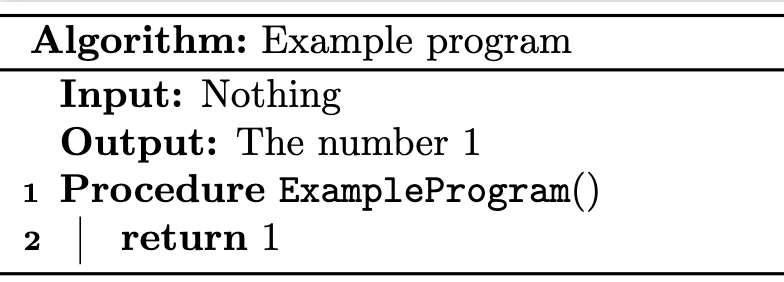
\includegraphics[scale=0.6]{assets/exampleProgramAlgorithm2e.png}
    \caption{The result of compiling \Cref{Example program with Algorithm2e to show macros in action.}}
    \label{The result of compiling Listing 4.10.}
\end{figure}

Another special macro is \texttt{\textbackslash SetKwFunction\{f\}\{f\}}. This allows us to write \texttt{\textbackslash f\{arg1, .., arg n\}}, to display \f{arg1, .., arg n} in the compiled version. \\

Since we are still in a LaTeX environment, and backslashes are used for macros in standard LaTeX too, we have to be careful. This is because we are not allowed to rename internal macros. For instance, \texttt{\textbackslash begin} is already a macro in LaTeX, thus attempting to compile a file with \texttt{\textbackslash SetKwFunction\{begin\}\{begin\}} will lead to multiple errors and ruin the final output.

\subsection{Compatibility with Psnodig}

As already mentioned in Section 4.2.2.3, all Psnodig library functions are taken into consideration by the TBP writer. The function call \texttt{length(list)} is transpiled with the cardinality symbols to \hspace{.01cm} $\abs{list}$. The function call \texttt{append(x, xs)} is transpiled to the natural language description \texttt{append x to xs}. \\

Mathematical expressions are also taken into account. For instance, the value \texttt{BinaryExp Division (Constant (Number 2)) (Constant (Number 1))} will show $\frac{2}{1}$, rather than something like \texttt{2/1}. Similarly, an expression with multiplication will be displayed as \texttt{m $\cdot$ n} rather than \texttt{m * n}. To work with mathematical symbols in LaTeX we use the packages \texttt{amsmath} and \texttt{commath}. They are always included, regardless of the rest of the program. \\

We also declare some macros to match the syntax of Psnodig. Before our programs are transpiled to TBP, we scan it for keywords, which are then reflected the LaTeX file. If our program contains code like \texttt{v := false}, the LaTeX file will include \texttt{\textbackslash SetKw\{False\}\{false\}}, and we will apply \texttt{\textbackslash KwFalse} rather than just ``false''.

\subsection{Output}

If we run \texttt{stack run tbp program} in our command line, and the program is syntactically correct, we receive a corresponding LaTeX file. If we add the \texttt{pdf} flag we also get a PDF of the compiled LaTeX file. \\

Just like the Gourmet writer, the TBP writer is not able to take the original source code's formatting into account. This means that a program like the one shown in \Cref{Gourmet f} will be transpiled to the one shown in \Cref{How Psnodig transpiles the program from} rather than the one shown in \Cref{Alternative version of f in LaTeX with Algorithm2e.}. \\

\begin{lstlisting}[caption={A Gourmet function which declares a variable and returns it.}, captionpos=b, label={Gourmet f}]
func f(){v:=5 returnv}
\end{lstlisting}

\begin{lstlisting}[caption={How Psnodig transpiles the program from \Cref{Gourmet f}.}, captionpos=b, label={How Psnodig transpiles the program from}]
\proc{$\f()$}{
    $\texttt{v} \gets 5$ \;
    \Return $v$ \;
}
\end{lstlisting}

\begin{lstlisting}[caption={Alternative version of f in LaTeX with Algorithm2e.}, captionpos=b, label={Alternative version of f in LaTeX with Algorithm2e.}]
\proc{$\f()$}{$\texttt{v}\gets5$\;\Return$v$;}
\end{lstlisting}

Even though the compiled versions produce the same PDF, we believe the curated amount of whitespace increases the maintainability of the LaTeX document, in case we wish to tweak it manually after transpilation. All transpiled documents will include \texttt{\textbackslash SetKwProg\{proc\}\{Procedure\}\{\}\{\}}, and the one transpiling \Cref{Gourmet f} will also have \texttt{\textbackslash SetKwFunction\{f\}\{f\}}. \\

We also import \texttt{linesnumbered} and \texttt{ruled} from Algorithm2e, purely for aesthetic reasons. \Cref{algoWithAndWithoutParams} shows two versions of \Cref{Gourmet f} after transpiling the source code and compiling the LaTeX. \Cref{f with linesnumbered and ruled.} has the parameters imported, whilst \Cref{f without plain Algorithm2e.} does not. \\

\begin{figure}[ht]
\centering
\begin{subfigure}{.5\textwidth}
  \centering
  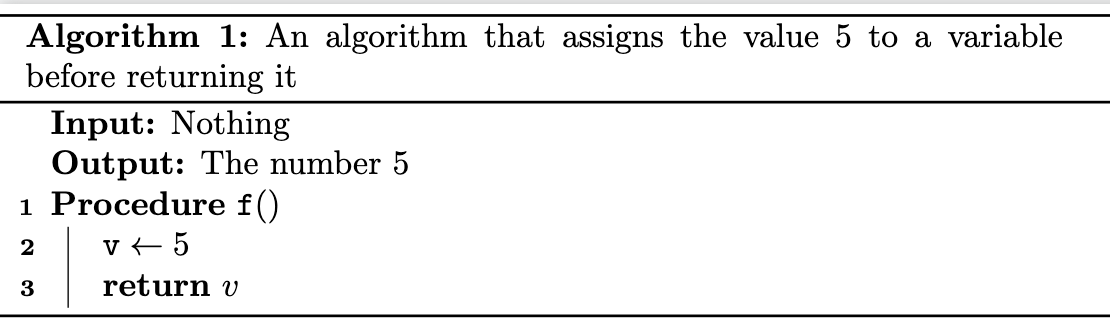
\includegraphics[width=.9\linewidth]{assets/return5pretty.png}
  \caption{\Cref{Gourmet f} with linesnumbered and ruled.}
  \label{f with linesnumbered and ruled.}
\end{subfigure}%
\begin{subfigure}{.5\textwidth}
  \centering
  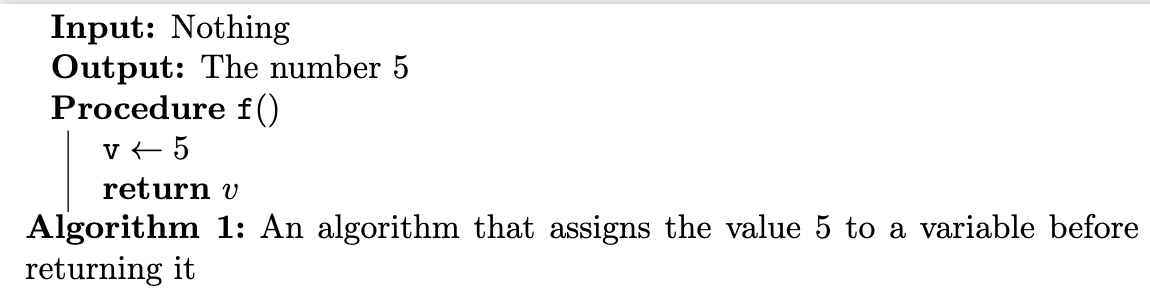
\includegraphics[width=.9\linewidth]{assets/return5ugly.png}
  \caption{\Cref{Gourmet f} without linesnumbered and ruled.}
  \label{f without plain Algorithm2e.}
\end{subfigure}
\caption{Compiled result of transpiling\Cref{Gourmet f}, with and without linesnumbered and ruled.}
\label{algoWithAndWithoutParams}
\end{figure}

Lastly, all documents transpiled to TBP include \texttt{\textbackslash DontPrintSemicolon} to prevent lines ending with semicolons, and \texttt{\textbackslash renewcommand\{\textbackslash thealgocf\}\{\}} to avoid numbering the compiled result. \Cref{algoWithAndWithoutParams} shows the result of including the latter. Since we only transpile the topmost function in a file, we feel like excluding the number looks cleaner. However, if we were to transpile multiple functions, it could make sense to remove it.

\section{Flowchart Writer}

Our third and last writer converts internal representations to LaTeX programs using the TikZ package. Compiling these files produce flowcharts. We believe there is value to working with such a different abstraction level (compared to Gourmet and TBP), and pretty flowcharts helps showcase Psnodig's powerfulness. \\

Just like the TBP writer, the IBP writer only works on topmost function in a file, ignoring the program description, structs and function call. Our reasoning is the same as earlier. \\

\subsection{TikZ}

TikZ is an enormous package, which can be used for just about anything related to drawing in LaTeX. In fact, we actually used TikZ to create the FSA example in \Cref{An example finite state automata.} \\

\forsup{Bør jeg skrive en intro om denne pakken også?}

Our flowcharts mainly consist of three macros: \texttt{\textbackslash tikzstyle}, \texttt{\textbackslash node}, and \texttt{\textbackslash edge}. \texttt{tikzstyle} lets us choose what our nodes look like, \texttt{node} lets us draw the nodes, and \texttt{edge} lets us add edges between nodes. \\

Each node in our flowcharts represents a statement, except the top one, which is the function name. The visual design is simple: the top node and all nodes of return statements are dark rectangles with rounded edges. Decision nodes, where the program diverges, are light yellow rectangles. This includes while-, for- and if-statements. The remaining statements are purple rectangles. Edges are thin arrows. \\

\Cref{Rough description of tikzstyle attributes.} gives a rough estimate of how a tikzstyle can be constructed. \\

\begin{lstlisting}[caption={Rough description of tikzstyle attributes.}, captionpos=b, label={Rough description of tikzstyle attributes.}]
\tikzstyle {unique name} =
    [ <shape>
    , minimum width = <x> cm
    , minimum height = <y> cm
    , text <position>
    , draw = <colour>
    , text = <colour'>
    , fill = <colour''>
    ]
\end{lstlisting}

Each style has a unique name, so that it can be applied to nodes later on.  The standard shapes are rectangles, circles and coordinates, however we can import libraries to get shapes like diamonds and ellipses. The three colours refer to a node's border-, text- and background colours, respectively. We have opted to center all text. \\

\Cref{How nodes are written with TikZ.} gives a rough estimate of how nodes are written. \\

\begin{lstlisting}[caption={How nodes are written with TikZ.}, captionpos=b, label={How nodes are written with TikZ.}]
\node (unique name)
      [metadata]
      {text displayed on node}
\end{lstlisting}

All nodes should have a unique name, so that they can be referenced correctly later. The square brackets denote metadata, like what the node should look like (by referencing a tikzstyle), or the node's positioning relative to other nodes. The curly brackets is the text displayed within the node body. \\

\Cref{How edges are written with TikZ.} shows how most edges are written. \\

\begin{lstlisting}[caption={How edges are written with TikZ.}, captionpos=b, label={How edges are written with TikZ.}]
\draw [edge] (node) -- (node')
\end{lstlisting}

\forsup{Eksempler?}

Additionally, having multiple straight edges from the same source might interfere with edge labels. Luckily, we can change the way we draw edges. For instance, we can change \texttt{$--$} to \texttt{$|-$}, like shown in \Cref{Alternative way of writing an edge.}. \\

\begin{lstlisting}[caption={Alternative way of writing an edge.}, captionpos=b, label={Alternative way of writing an edge.}]
\draw [edge] (node) |- (node');
\end{lstlisting}

This will curve the edge between \texttt{node} and \texttt{node'}, making the flowchart clearer. However, knowing when to use which kind of edge is difficult since we never know how programs turn out beforehand. Therefore, we usually stick to \texttt{$--$}. If we are left dissatisfied with the result, we can always tweak the LaTeX file later on.

\subsection{Compatibility with Psnodig}

To make the corresponding flowcharts clear as well as pleasing, we have opted for three different node themes. This will make it easier to differentiate significant contexts. \\

The start node and all return nodes have the same theme of rectangles with white text on a dark background. Statements containing a list of statements have the same theme of ellipses with black text on a yellow background. Lastly, all remaining statements have the theme of rectangles with black text on a light purple background. \Cref{flowchartColours} shows the result of transpiling a simple function, showcasing all the aforementioned node styles. \\

\begin{figure}[ht]
    \centering
    \includegraphics[scale=.5]{assets/def_FlowchartColours.png}
    \caption{A program showcasing all the different node types the Flowchart generator produces}
    \label{flowchartColours}
\end{figure}

Just like the TBP writer, the IBP writer uses mathematical notation where appropriate. For instance, \texttt{x \&\& y} is transpiled to \texttt{x $\land$ y}. Contrary to the TBP writer however, Psnodig's library functions are not considered. That means that code like \texttt{length(collection)} will look identical both in the source code and the corresponding flowchart. \\

There are a few design choices worth noting. Return expressions do not explicitly say \texttt{return}, as their context is given by the node theme. Also, recursive function calls do not have an arrow back to the original node stating the function name, but are instead written as their own nodes. For one, there is no straightforward way of creating arrows on this form with TikZ, but we also believe a flowchart with too many arrows looks confusing. \\

All statements are displayed in a simple rectangular box, but \texttt{Loop}-, \texttt{ForEach}-, \texttt{For}-, and \texttt{If}-statements are - as previously mentioned - given their own node themes. This is because they break with the standard linear pattern, and contain statements of their own. \\

\texttt{\textbf{For} identifier from to statements} starts with assigning \\ \texttt{identifier} to \texttt{fromRange}. The next node is a light yellow rectangle. If \texttt{from} and \texttt{to} are both numericals, the rectangles text will be either \texttt{from < to ?} or \texttt{from > to ?}, depending on their values. If they are not both numericals, the default is \texttt{from < to ?} since we do not evaluate expressions, and have no way of knowing their actual values. \\

From this light yellow rectangle, we have an edge labeled \texttt{true} which points to the next statement \textit{after} the current \texttt{\textbf{For}} (if there are any). In the opposite way, an edge labeled \texttt{false} points to the first statement in \texttt{statements}. After the last of these, there is an assignment statement, either incrementing or decrementing \texttt{identifier}, before pointing back to the light yellow rectangle. \\

\Cref{forExample1}, \Cref{forExample2}, and \Cref{forExample3} shows the three different ways a \texttt{\textbf{For}}-statement can be transpiled to a flowchart. \\

\begin{figure}[ht]
    \centering
    \includegraphics[scale=.38]{assets/def_ForExample2.png}
    \caption{A \texttt{For}-statmenet where \texttt{from < to}.}
    \label{forExample1}
\end{figure}

\begin{figure}[ht]
    \centering
    \includegraphics[scale=.38]{assets/def_ForExample3.png}
    \caption{A \texttt{For}-statmenet where \texttt{from > to}.}
    \label{forExample2}
\end{figure}

\begin{figure}[ht!]
    \centering
    \includegraphics[scale=.38]{assets/def_ForExample2.png}
    \caption{A \texttt{For}-statmenet where \texttt{from} and \texttt{to} are not both numericals.}
    \label{forExample3}
\end{figure}

\forsup{Bør disse heller spares til Evaluation?}

\texttt{\textbf{ForEach} identifier collection statements} starts with a light yellow rectangle asking if we have iterated \texttt{collection}. From here there are two arrows. The first is labeled \texttt{true} and points to the next statement after the current \texttt{\textbf{ForEach}} (if there are any). \\

The other one is labeled \texttt{false} and points to a statement stating \texttt{identifier $\gets$ next element in collection}. Then each statement in \texttt{statements} is presented. After the last of these, there is an arrow pointing back to the light yellow rectangle. A working example is presented in \Cref{flochartForEach}. \\

\begin{figure}[ht]
    \centering
    \includegraphics[scale=0.39]{assets/def_ForEachExample.png}
    \caption{A \texttt{ForEach}-statement, iterating a variable \texttt{teams}.}
    \label{flochartForEach}
\end{figure}

\texttt{\textbf{While} condition statements} largely follows the pattern of \texttt{\textbf{ForEach}}. The statement starts with a light yellow rectangle displaying \texttt{condition} followed by a question mark. \\

There are again two edges: The first is labeled \texttt{true} and points to the next statement after the current \texttt{\textbf{While}} (if there are any). The other is labeled \texttt{false} and points to the first statement in \texttt{statements}. The last of these points back to the light yellow rectangle. A working example is presented in \Cref{flochartWhile}. \\

\begin{figure}[ht]
    \centering
    \includegraphics[scale=0.39]{assets/def_WhileExample.png}
    \caption{A \texttt{While}-statement, iterating until \texttt{i} reaches the value of \texttt{bigNumber}.}
    \label{flochartWhile}
\end{figure}

\texttt{\textbf{If} condition statements else} is the most intricate statement of the four discussed in this section. Again we start with a yellow rectangle displaying \texttt{condition} followed by a question mark. An edge labeled \texttt{true} points to the first statement in \texttt{statements}. Another edge labeled \texttt{false} points to either \texttt{else}, the next statement after the current \texttt{\textbf{If}}, or nothing, since both are optional. \\

If last statement in \texttt{statements} is not a \texttt{Return}-statement, it must point to the next statement outside the current \texttt{\textbf{If}} (if there is one). If \texttt{else} is present, the same applies to its statement list. \\

If the last statement in \texttt{statements} is a \texttt{Return}-statement, and the same is the case for all subsequent \texttt{else}s, the next statement after the current \texttt{\textbf{If}} is unreachable. If our code still has this structure, we are told in the command line, and the transpilation is interrupted. \\

\forsup{Her skal jeg vise en del eksempler}

\subsection{Output}

Transpiling IBP with the command line works precisely like it does with TBP. We run \texttt{stack run ibp program} to transpile the program and receive a corresponding LaTeX file, given that the program is syntactically correct. If we also wish for the compiled result, we add a \texttt{pdf} flag. \\

\Cref{Example output from compiling Flowchart} shows the (most important parts of the) LaTeX file we receive by transpiling the program in \Cref{Gourmet f}. We see how every node has a unique id, reference a tikzstyle, and how the metadata describes their placement. We also make a point out of drawing all the edges \textit{after} drawing all the nodes, for the sake of readability. To take this one step further, we also sort the edges on the id of the source node. \\

\begin{lstlisting}[caption={Excerpt of the LaTeX from transpiling \Cref{Gourmet f} to IBP.}, captionpos=b, label={Example output from compiling Flowchart}]
\node (0) [startstop] {f()};
\node (1) [statement, below of=0] {v = 5};
\node (2) [startstop, below of=1] {v};

\draw [edge] (0) -- (1);
\draw [edge] (1) -- (2);
\end{lstlisting}
